\documentclass[a4paper,10pt]{scrartcl}
\usepackage[german,ngerman]{babel}
\usepackage[utf8]{inputenc}
\usepackage[T1]{fontenc}
\usepackage{lmodern}
\usepackage{fullpage}
\usepackage{tikz}
\usepackage{multicol}
\usepackage{wrapfig}
\usepackage{droid}
\usepackage{tabularx}
\usepackage[colorlinks, pdfpagelabels, pdfstartview = FitH, bookmarksopen = true,bookmarksnumbered = true, linkcolor = black, plainpages = false, hypertexnames = false, citecolor = black] {hyperref}

\graphicspath{{images/}}

\author{Zusammengetragen von einem Subset des inf12-Jahrgangs}
\title{Was man über IKON 2 wissen muss}
\date{Viel zu kurz vor der Klausur}

\pagestyle{plain}

\renewcommand{\headheight}{12pt}
\renewcommand{\headsep}{12pt}

\setlength{\parindent}{0pt}
\setlength{\parskip}{0.6em}
\linespread{1.2}

\begin{document}
\setcounter{secnumdepth}{0}

\maketitle
\tableofcontents
\newpage

\section{VL 01: Motivation}
In dieser Vorlesung geht es im Prinzip darum, dass der Kontext wichtig für Informatiker ist, da:
\begin{itemize}
	\item Informatik den Kontext verändert
	\item Informatik Teil des Kontextes ist
	\item Informatik neue Kontexte schafft
	\item Kontexte die Informatik verändern
\end{itemize}
Kontexte können sein:
\begin{itemize}
	\item Gesellschaft
	\item Organisationen
	\item Geschäftsmodelle / -prozesse
	\item Dienstleistungen
	\item Individuen
\end{itemize}

Informatiker müssen den Kontext \em dekontextualisieren\em, d.h. ihn \em verstehen, analysieren und modellieren \em können. Anders herum müssen sie auch Informatiksysteme \em rekontextualisieren \em, d.h. sie \em verändern, einführen und warten \em können.
\section{VL 02: Welchen nutzen stiftet IT in Organisationen?}
Thema: Wofür werden Informationssysteme in Unternehmen eingesetzt und was bewirkt das?

Informationssysteme
\begin{itemize}
	\item Informieren
	\item Erleichtern die Kommunikation
	\item Koordinieren
	\item Automatisieren
\end{itemize}

Wichtige Definitionen:
\begin{description}
	\item[Unternehmung] Ein \em Betrieb \em in einem marktwirtschaftlichen System.
	\item[Betrieb] Eine planvoll organisierte Wirtschaftseinheit, in der Produktionsfaktoren kombiniert werden, um Güter und Dienstleistungen herzustellen und abzusetzen.
	\item[Informationssystem] Soziotechnische (Mensch \em und \em Maschine) Systeme, die der optimalen Bereitstellung von Information und Kommunikation nach wirtschaftlichen Kriterien dienen.
\end{description}

Organisation mit Informationssystem:
\begin{center}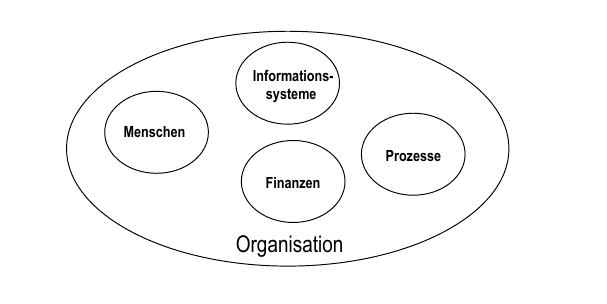
\includegraphics[width=0.8\textwidth]{IS-Kontext.png}\end{center}

In vielen Diagrammen und Studien kann man sehen: IT wirkt stark zeitversetzt und (fast nur) in Verbindung mit einer Dezentralisierung der Organisationsstruktur.

Der Nutzen von Informationssystemen in Unternehmungen wird durch folgendes Diagramm zusammengefasst:

\begin{center}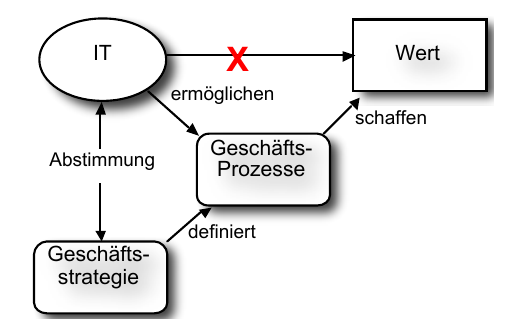
\includegraphics[width=0.9\textwidth]{IS-Nutzen.png}\end{center}

Die Beispiel-Klausuraufgabe war, dieses Diagramm zu beschriften.
\section{VL 03: <title>}

\section{VL 04: Kontext Organisation}

\textbf{Organisation:} Ordnung, die zielgerichtet arbeitsteilig Aufgaben und
Tätigkeiten regelt. -- Zweckorientiertes soziales Gebilde.

Eine Organisation muss \textbf{Koordinieren}, \textbf{Motivieren}, und eigentlich auch
Orientieren (Knowledge Sharing), aber darum geht's nicht in IKON.

Dazu gehört Arbeitsteilung -- \textbf{horizontale Arbeitsteilung} nach Projekten, Regionen, Objekten und Funktionen,
\textbf{vertikale Arbeitsteilung} heißt auch ,,Hierarchie''.

\subsection{Koordination}

\begin{description}
    \item[Leitungsbeziehungen] Wer darf wen kommandieren?
    \item[Standardisierung] Generelle Regelungen
    \item[Delegation] Du machst das!
    \item[Partizipation] Wir bauen zusammen was tolles...
\end{description}

\subsection{Motivation}

\begin{description}
    \item[Extrinsisch] Belohnung / Bestrafung (finanziell oder reputationell) / Zielvereinbarung
    \item[Intrinsisch] Individuelles Bestreben, Interesse, ...
\end{description}

\begin{center}{\large Bestimmt IT unser Handeln \emph{oder} bestimmt unser Handeln die IT?}\\
{\footnotesize Antwort vom Troll-Prof: Beides! 
\includegraphics[width=0.3cm]{wichtige-anmerkung.png}}\end{center}

Weiterer Vorlesungsinhalt: Open Source ist awesome! Und funktioniert nur wegen IT (CVS, Mail, Bugtracker, Github!).

\subsection{Technochange}

\begin{center}{\large \emph{Zusammenspiel} zwischen IT und \emph{Organisations}veränderung.}

... aka neue Technik, die Geschäftsprozesse etc. beeinflusst.
\end{center}

\section{VL 05: Kontext Prozess I}

BPMN (Business Process Model Notation): Ansatz zur Prozessmodellierung

\begin{itemize}
  \item Prozess: Eine Folge von logischen Einzelfunktionen, zwischen denen Verbindungen bestehen. Dabei gibt es einen Auslöser der den Prozess ggf. mit Input startet.
  \item Prozessmanagement: Gestaltung, Ausführung und Beurteilung von Funktionsfolgen (Prozesse)
\end{itemize}


\subsection{Prozessmodelle}

\begin{itemize}
  \item Darstellung der Abfolgen und Verantwortlichkeiten – es lassen sich auch fehlerhafte Prozesse dokumentieren und verbessern
  \item BPMN ist ein bekannter Modellierungsansatz
\end{itemize}

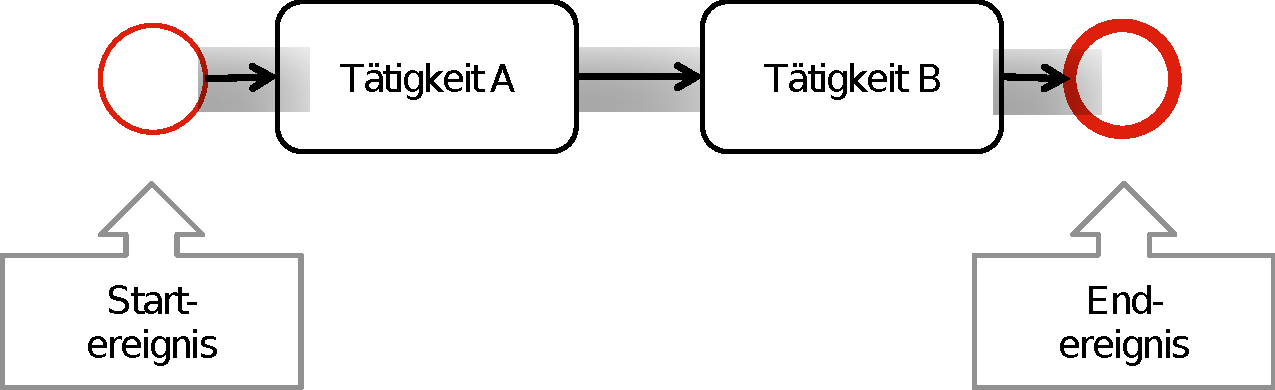
\includegraphics[width=0.7\textwidth]{5-1}

\begin{itemize}
  \item Nomen \& Verben: Was wird wie gemacht/verändert? Die Aktivitäten werden als Kästchen darstellt.
  \item Sequenzfluss: Welche Reihenfolge hat eine Tätigkeit? Die nächste Aktivität wird erst gestartet, wenn die vorherige Aktivität beendet wurde.
  \item Ereignisse: Trigger/Auslöser des Prozesses – als Kreise im Prozessdiagramm
\end{itemize}

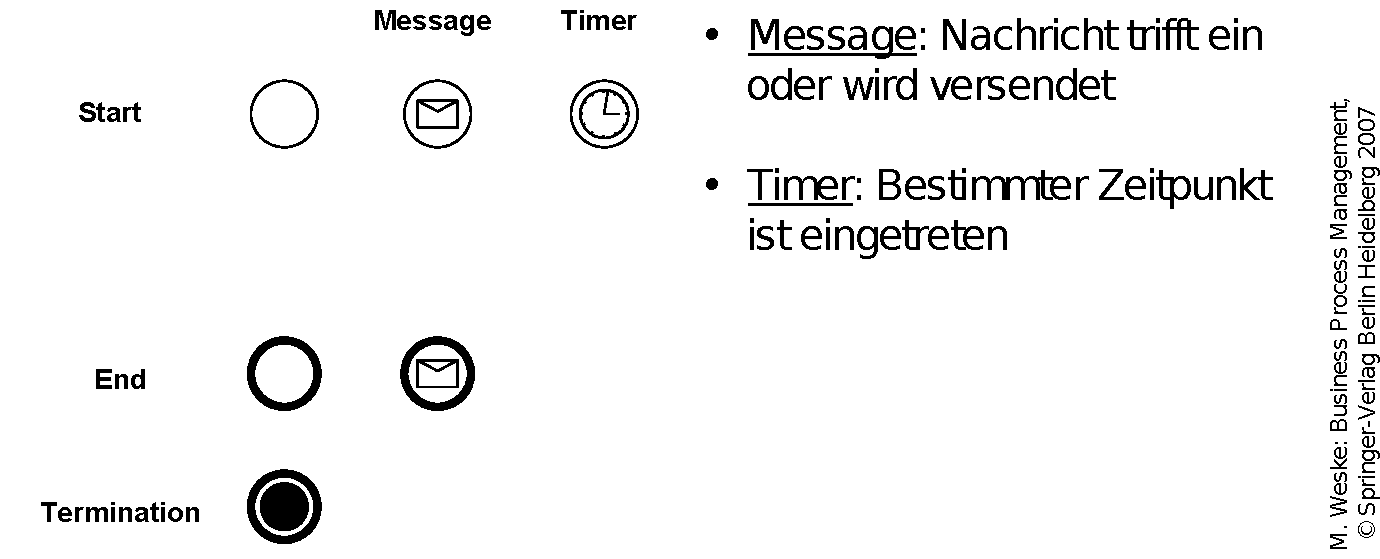
\includegraphics[width=\textwidth]{5-2}


\subsubsection{Swimmlanes und Pools}

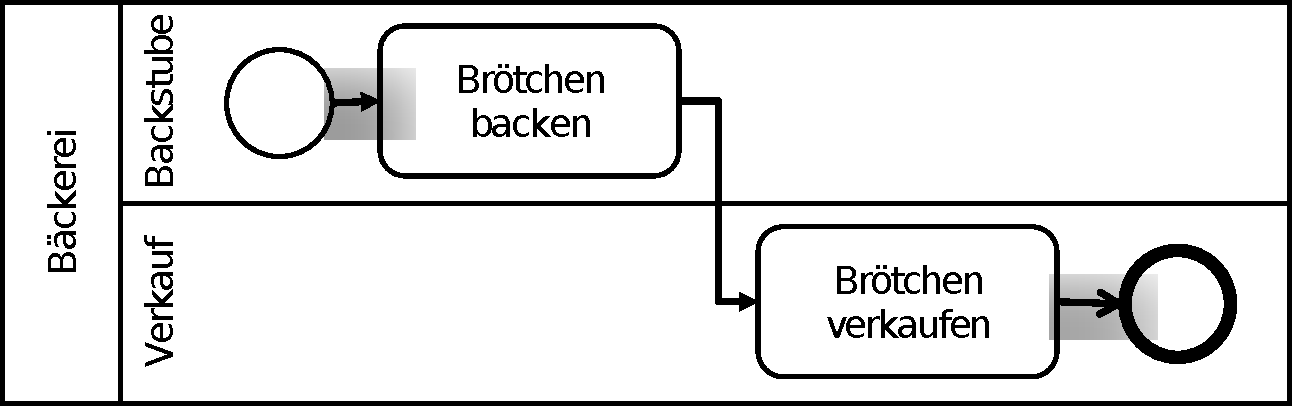
\includegraphics[width=0.7\textwidth]{5-3}

\begin{itemize}
  \item Pool ist ein Beteiligter (z.B. eine Organisation) [Bäckerei]
  \item Swimlane representiert eine Untergruppe, welche in Organisationen eingereiht werden [Verkauf, Backstube]
\end{itemize}


\subsubsection{Gateways}

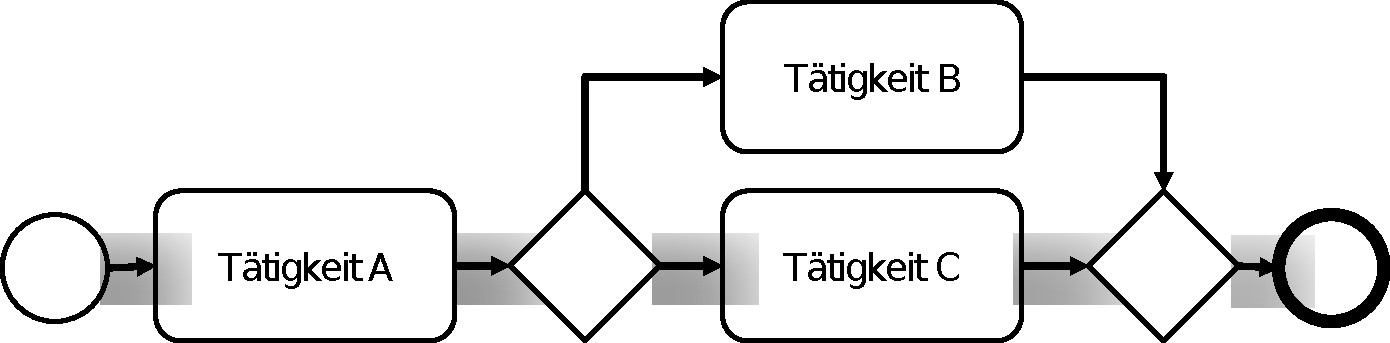
\includegraphics[width=0.7\textwidth]{5-4}

\begin{itemize}
  \item Sind eine Verzweigung der Aktivitätsfolge
  \item Regeln nach denen Prozesse ablaufen/gesteuert werden, z.B. zur Parallelisierung
  \item Exclusive Gateways: Je nach Bedingung genau eine Kante als Ausgabe. Gleiches gilt bei Zusammenführung – es muss nur eine einlaufen.
\end{itemize}

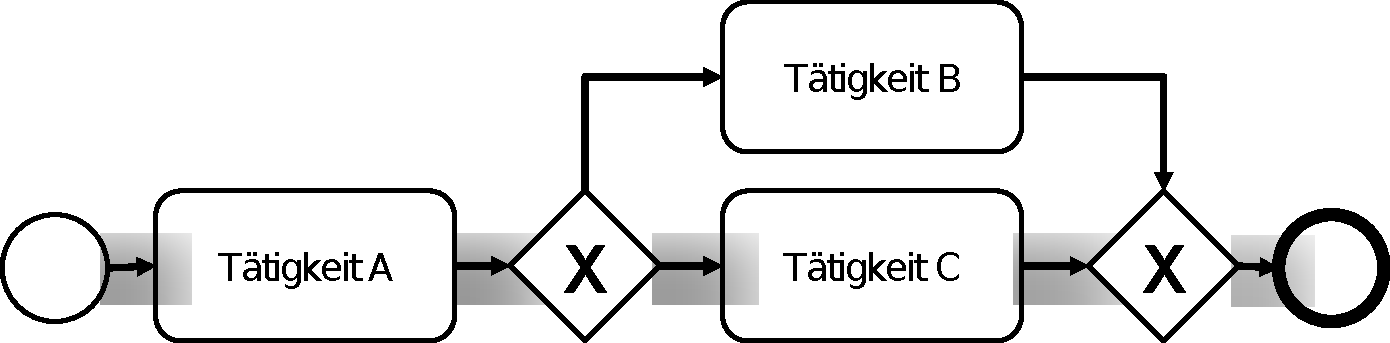
\includegraphics[width=0.7\textwidth]{5-5}

\begin{itemize}
  \item Parallele Gateways: Beide Aktivitäten werden gestartet. Beim Zusammenführen wird auch auf alle Fertigstellungen gewartet.
\end{itemize}

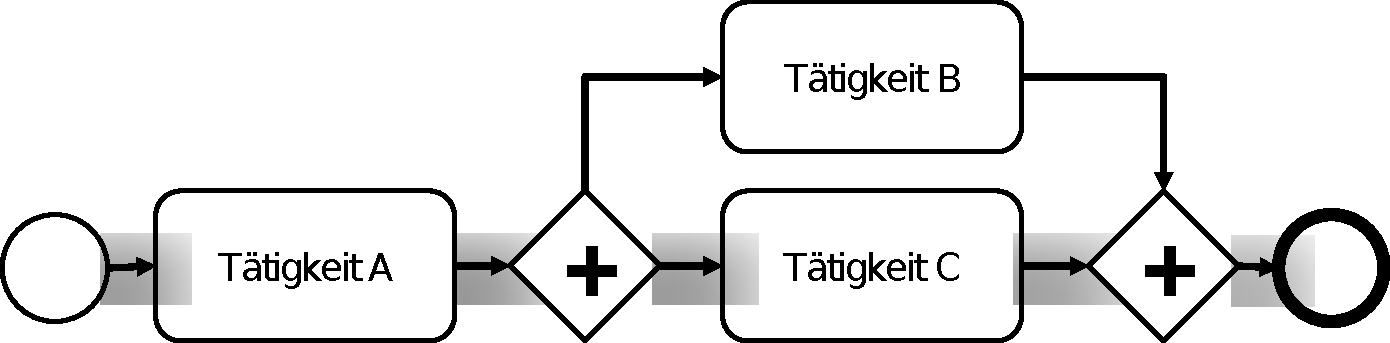
\includegraphics[width=0.7\textwidth]{5-6}
\section{VL 06: Kontext Prozess II}

\subsection{Nachrichtenfluss}

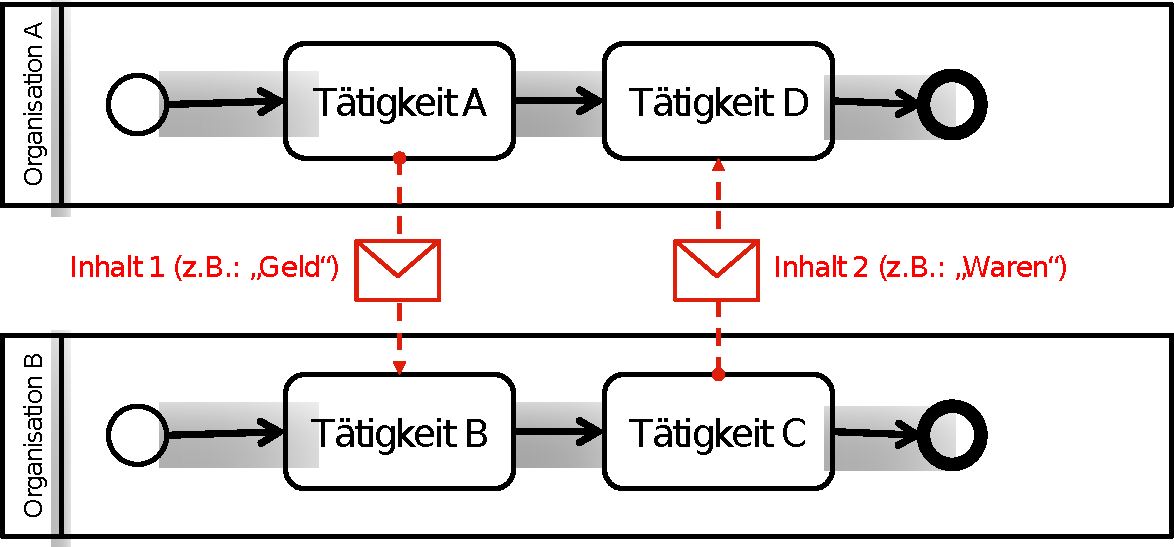
\includegraphics[width=0.7\textwidth]{6-1}

\begin{itemize}
  \item Informationsaustausch zwischen unterschiedlichen Organisationen
  \item Ein gestrichelter Pfeil A $\rightarrow$ B bedeutet dabei, dass B auf eine Nachricht von A wartet
  \item »Das Einführen von Swimlanes ist durchaus mit dem Malen von Kästchen verbunden«
\end{itemize}


\subsection{Prozessmodell am Beispiel Pizza}

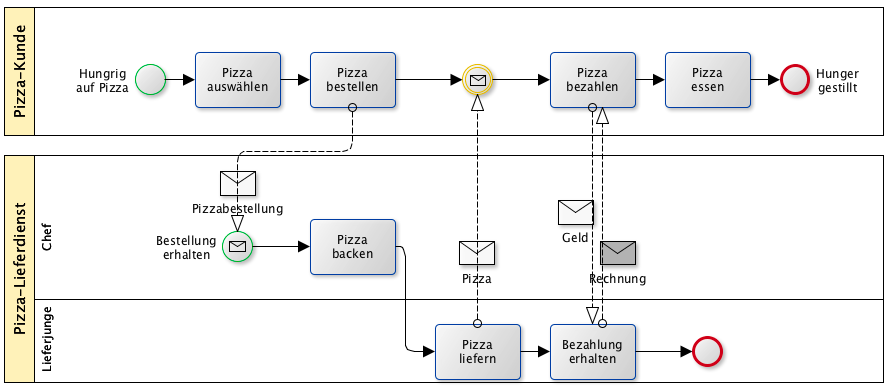
\includegraphics[width=\textwidth]{6-2}

Ein weiteres Beispiel-Modell zu Prozessmodellen (Logistik) findet sich im Foliensatz.


\subsection{Verbesserungen von Prozessmodellen}

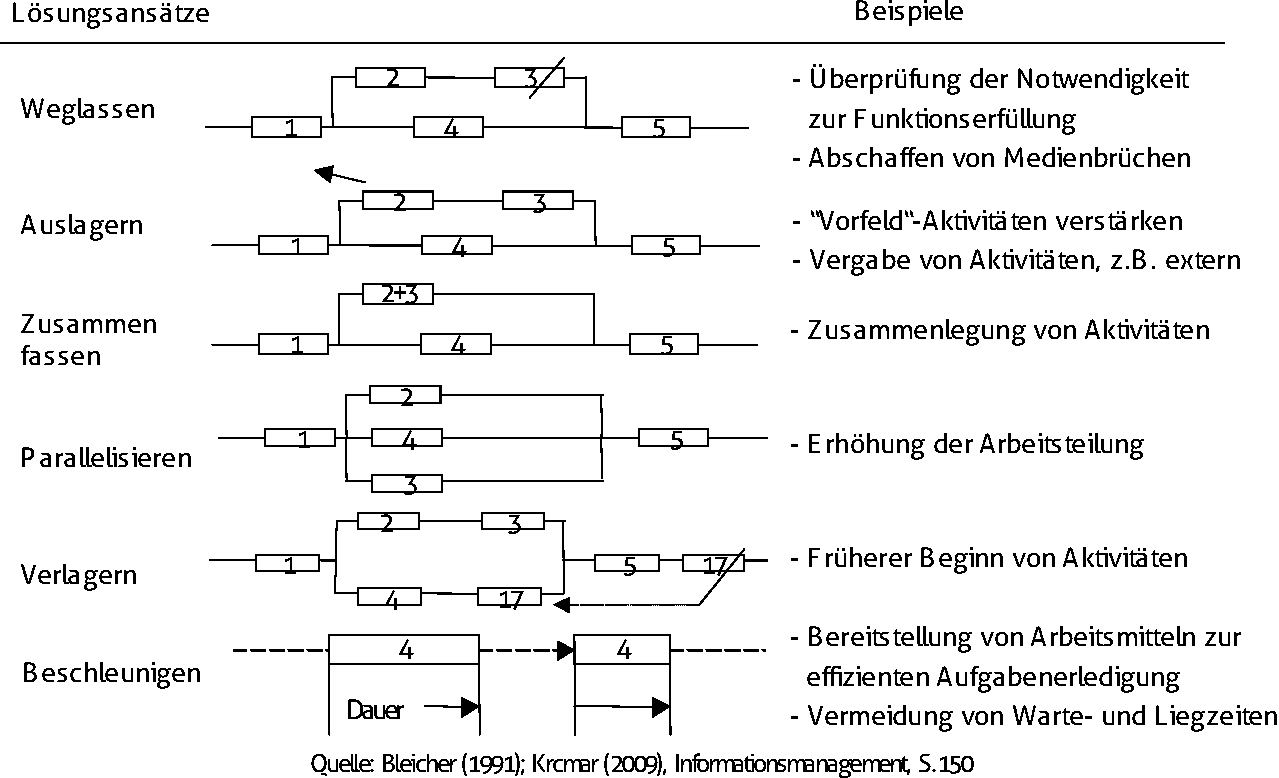
\includegraphics[width=\textwidth]{6-3}


\subsection{IT-Potenziale zur Prozessverbesserung}

\begin{tabularx}{\textwidth}{|l|X|} \hline
  IT-Potenzial     & Organisatorischer Einfluss/Nutzen \\\hline\hline
  Automatisch      & Reduktion manueller Eingriffe und Standardisierung der Prozesse \\\hline
  Informativ       & Verfügbarkeit großer Mengen detaillierter Informationen \\\hline
  Sequenziell      & »natürliche« Reihenfolge der Aktivitäten bis zur Parallelisierung \\\hline
  Zielorientiert   & Kontinuierliche Verfolgung des Prozessstatus \\\hline
  Analytisch       & komplexe Auswertung vorhandener Informationen \\\hline
  Geographisch     & Unabhängigkeit von räumlichen Gegebenheiten \\\hline
  Integrierend     & Zusammenfassung auch heterogener Aufgaben \\\hline
  Wissen schaffend & flächendeckende Verfügbarkeit von Wissen und Expertise \\\hline
  Vereinfachend    & Entfernung von Intermediären aus dem Prozess \\\hline
\end{tabularx}

\newpage
\section{VL 07: Kontext Individuum -- Technologieakzeptanz}

\begin{multicols}{2}
Wesentlich im Lebenszyklus eines Informationssystems ist die Einführung - hier entscheidet
sich der Erfolg und die Bedeutung. Damit Informationssysteme \textbf{Nutzen} stiften können,
müssen sie (korrekt) \textbf{genutzt} werden:

\begin{center}{\large,,Vor dem \emph{Nutzen} kommt die \emph{Nutzung}.''}\end{center}

Um Akzeptanz und Verständnis zu erreichen, ist ein geplanter \textbf{Einführungsprozess}
des Systems innerhalb der Organisation notwendig.

\begin{center}{\textbf{Einführung von Informationssystemen}:\\
Eine organisatorische Maßnahme zur Verbreitung (Installation) und\\
Aneignung (Verwendung) von Informationstechnik in einer Nutzergruppe.}\end{center}

Wie breitet sich eine Innovation aus? Rogers Prozess der \textbf{Diffusion:} Mitglieder eines
sozialen Systems kommunizieren über verschiedene Kanäle $\Rightarrow$ Es muss über die
Innovation gesprochen/geschrieben werden.
\\
\\

\begin{center}
\textbf{Schritte der Aneignung einer Innovation}\\
Wissen (\emph{aha, sowas gibts!})\\
Überzeugung (\emph{das klingt gut!})\\
Entscheidung (\emph{ich probier das aus})\\
Umsetzung (\emph{click here to download, next, agree, next, next, finish})\\
Bestätigung (\emph{is ja echt voll geil!})
\end{center}

Merkmale des Individuums beeinflusses sein Wissen, Merkmale der Innovation beeinflussen
seine Überzeugung. Der Kommunikationskanal muss auf die Zielgruppe angepasst werden.

\textbf{Innovationsfreudigkeit}\\
2.5\% Innovatoren\\
13.5\% Frühe Nutzer\\
34\% Frühe Mehrheit\\
34\% Späte Mehrheit\\
16\% Nachzügler

\textbf{Innovations-Merkmale nach Rogers:}\\
\emph{Wahrgenommener} Vorteil\\
Komplexität (\emph{vs. Einfachheit})\\
Kompatibilität (\emph{technisch, sozial, ...})\\
Beobachtbarkeit (\emph{Preview bei anderen})\\
Probierbarkeit (\emph{Demo-Version etc.})
\end{multicols}

Leistungserwartung + Aufwandserwartung + Sozialer Einfluss = Nutzungsintention

Nutzungsintention + Fördernde Bedingungen = Nutzungsverhalten

Ansonsten gibt's immer \emph{Moderatorgrößen}, die ,,halt einfach noch eine
Rolle spielen'' (so wie das Wetter den Genuss beim Eis-Essen beeinflusst). Typische
Faktoren: Alter, Geschlecht, ... .

\section{VL 08: Kontext Markt}
IT Dienstleistungen und Cloud Computing

Der IT-Markt besteht aus Software, Hardware und IT-Dienstleistungen, wobei die Kategorie Software noch einmal in die Unterkategorien System-Infrastruktur, Werkzeuge und Anwendungs-Software unterteilt werden kann.

\begin{itemize}
\item IT-Leistungen werden zum Teil an andere Unternehmen weitergeleitet, falls das billiger ist, als es selbst zu machen (= Outsourcing). Das geht in jedem Bereich des IT-Marktes.
\item In jedem Unternehmen wird Software anders gehandhabt: Manche entwickeln alles selbst, andere setzen auf Standardsoftware und Dienstleistungen. Der Trend geht allerdings zur Standardsoftware mit Dienstleistungen hin
\item Trend hin zu Cloud-Diensten ( "Public Cloud" ): 
\begin{itemize}
\item "Kann ich nicht statt den Einzelteilen gleich das fertige Paket haben?"
\item Kapazität einfach bestellbar ohne Zusatzaufwand
\item Für die Anbieter: Optimalere Auslastung durch Nutzergruppen in verschiedenen Zeitzonen
\item Große Rechenzentren an Orten mit Kostenvorteilen (Antarktis -> Kühlung)
\item Bei großen Unternehmen kann man beide Seiten intern kombinieren: "Private Cloud"
\end{itemize}
\item Hypes verlaufen in einer $\sim$ -Kurve. Siehe dazu den "Gartner Emerging Technologies Hype Cycle".

\end{itemize}
\section{VL 09: Kontext Gesellschaft}
Informatik und Gesellschaft sind verzahnt!

\subsection{Definition Gesellschaft:}
Zwei Theorien:
\begin{itemize}
	\item Emile Durkheim:
	Die Gesellschaft beeinflusst und prägt das Individuum. 
	\item Max Weber:
	Gesellschaft ensteht durch individuelle Handlungen.
\end{itemize}
Die Emile Durkheim und Max Weber Definitionen setzen sich zusammen zu der Folgenden:

\emph{,,Gesellschaft = durch veränderliche, unterschiedliche Merkmale (Strukturen)
zusammengefasste und abgegrenzte Anzahl von Personen, die als soziale
Akteure miteinander verknüpft leben und direkt oder indirekt interagieren
(Handlungen) (Wikipedia 2012, mit Ergänzungen (in rot))''}


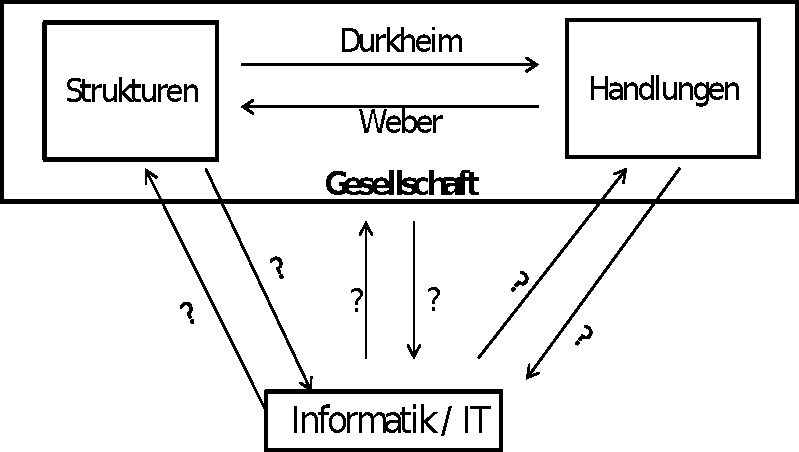
\includegraphics[width=0.7\textwidth]{9-1}

\subsection{Welchen Einfluss hat IT also auf Gesellschaft, Strukturen und Handlungen?}

\begin{itemize}
\item Handlungen: 
	\begin{itemize}
		\item Wie bei Individuen bereits geklährt.
	\end{itemize}
\item Gesellschaft:
	\begin{itemize}
		\item Grundrecht informationelle Selbstbestimmung (Datenschutz):
			\begin{itemize}
				\item Grundrecht ging aus Volkszählung hervor, 1983 entschied Bundesverfassungsgericht, das es dieses Grundrecht durchs Grundgesetz (freie Entfaltung) impliziert wird.
				$ \rightarrow $ Datenschutz in Deutschland wird gefestigt 
				\item Datenvermeidung %& Sparsamkeit. (bisweilen in der Praxis nicht umgesetzt)
			\end{itemize}
		\item Bild der Informatik
			\begin{itemize}
				\item Typisches Klischee (Nerd)
				\item zugleich sehr gesuchte Berufsgruppe.
			\end{itemize}
	\end{itemize}

\item Strukturen beeinflussen die Informatik:
	\begin{itemize}
		\item Gesetze
		\item Werte, Kultur, Leitbilder 
		\item Arbeitsmarkt
	\end{itemize}
\item Informatik beeinflusst Strukturen:
		\begin{itemize}
		\item Web 2.0:
			\begin{itemize}
			\item Verändert Freizeitverhalten
			\item Arab Spring etc.
			\item Freiheit von Informationen etc.
			\item Internetsucht
			\end{itemize}
		\end{itemize}
\end{itemize}

Insgesamt beeinflusst Informatik die Strukturn durch neue Technologien und Innovationen sowie durch optimierte Prozesse (z.B. Technochange)

Dadurch das Handlungen und Struckturen durch IT beeinflusst werden verändert sich entsprechend auch die gesamte Gesellschaft.
\section{VL 10: Kontexte verändern sich}

\newpage
\section{VL 11: Kontexte sind verzahnt - GreenIT}

Harald Welzer, spiegel online: So kann es nicht weitergehen, ökologisch und
finanziell. Ressources werden zur Neige gehen.  Klimawandel ist Scheiße --
deshalb müssen wir weniger Strom verbrauchen.

Leider ist wirtschaftliche Entwicklung regional orientiert. ,,Sollen doch die anderen
machen!'' Hippies haben in den 80ern angefangen mit \emph{Recycling}. Das war mega
cool (Kreislaufwirtschaft)! Und in den 90ern haben auch Unternehmen möglichst
Müll-effizient (ökologische Nachhaltigkeit) zu \emph{produzieren}.

Es wird immer mehr Energie verbraucht (wirklich? Wahnsinn!). Warum handeln Unternehmen
jetzt?

\begin{enumerate}
\item Treibhausgase und Ressourcen einsparen (\emph{ökologisch}, wie langweilig)
\item Geld sparen, weil Energie immer teurer wird (\emph{ökonomisch}, yay, Wirtschaft!)
\end{enumerate}

Seit 2008 wird von Unternehmen versucht, viel Strom in IT zu sparen, insbesondere
im Serverbetrieb. Einige sagen, ,,GreenIT'' sei nur ein Deckmantel, um neue (stromsparende) Hardware
zu verkaufen, aber neue Hardware herzustellen koste viel mehr Strom, als sie im
Endeffekt einspart. Man muss beide Seiten betrachten:

\begin{multicols}{2}
\subsection{GreenIT im engeren Sinne}

\begin{itemize}
\item Sparsame Hardware
\item Thin-Clients
\item effizientere Kühlsysteme
\item Energieoptionen, Herunterfahren!
\item ökologisches Design
\item Server-Virtualisierung
\end{itemize}

\subsection{GreenIT im weiteren Sinne}

\begin{itemize}
\item Herstellung von Hardware (Rohstoffe, Chemikalien, Energie)
\item Entsorgung von Hardware (Recyclingaufwand)
\item Energieaufwand für Betrieb (siehe oben)
\item Software-Hardware-Beziehung (braucht man wirklich neue Hardware?)
\end{itemize}
\end{multicols}

Und bitte, schickt nicht die alten Computer nach Afrika zu armen Kindern zum Recycling!
Das ist ungesund und schlecht für die Umwelt.

\subsection{Dematerialisierung und Reboundeffekt}

\textbf{Dematerialisierung:} Ein vorher physisch vorhandenes Objekt wird mit neuer Technologie weniger/kleiner oder
fällt weg. Beispiele: elektronische Dokumente, mp3-Download statt CD kaufen.
$\Rightarrow$ \textbf{Erhöhung der Ressourcenproduktivität}

\textbf{Reboundeffekt:} Weil Dinge Ressourcen sparen, werden sie günstiger, deshalb werden mehr genutzt, und
wieder mehr Ressourcen verbraucht. Beispiel: früher gabs ein paar große Mainframes, dann kamen
PCs, jetzt gibts davon Millionen.

Software kann solche Dinge modellieren und beim Ressourcen sparen/Klimaschutz helfen. Yay!

\section{VL 12: Kontexte sind verzahnt: Social Media}

\textbf{Web 2.0}, das Web wird als Plattform benutzt, auf der alle Benutzer Inhalte
gemeinsam verändern und hinzufügen.

\textbf{Social Media}, eine Gruppe von Webanwendungen, die auf Web 2.0 aufbauend
den Nutzern \emph{Herstellung} und \emph{Austausch} digitaler Inhalte (\emph{User
Generated Content}) ermöglichen.

\begin{itemize}
\item Peer-to-Peer Kommunikation
\item User Generated Content
\item Einfachheit der Nutzung
\item Hohe Verfügbarkeit (jeder, überall, jederzeit)
\item Öffentliche Handlungen
\end{itemize}

\textbf{Früher} (Web 1.0): IT hat Geschäftsprozesse ermöglicht und angetrieben

\textbf{Heute} (Web 2.0): Hohe Nutzerzahlen treiben den Fortschritt an, IT setzt um.

\subsection{Anwendungsklassen von Social Media}

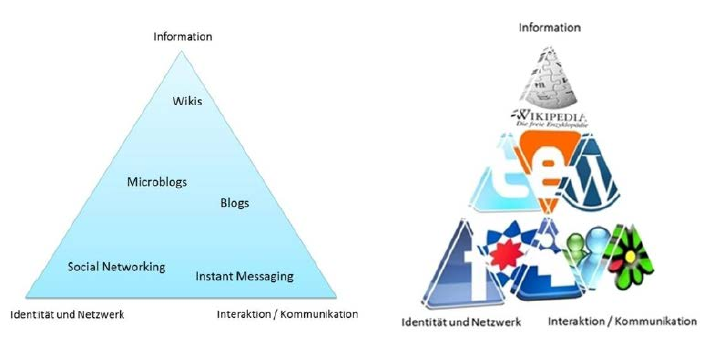
\includegraphics[width=0.9\textwidth]{anwendungsklassen.png}

Einteilung: Private (Facebook etc.) / Business/Professional (LinkedIn...) / Specialized (Github!)

\subsection{Enterprise 2.0}

Enterprise 2.0 ist die Nutzung von Social Media entweder \emph{innerhalb einer
Organisation} oder \emph{als Verbindung zu Partnern und Kunden} $\Rightarrow$ offene
Innen- und Außenkommunikation.

\textbf{Interne Nutzung}: Zusammenarbeit, Austausch von Wissen, Verbesserung von Prozessen.

\textbf{Externe Nutzung}: Marketing, Imagebildung, Recruiting, Zusammenarbeit mit Experten / Zulieferern.
\newpage

\section{VL 13: IT und Frauen}


\subsection{Warum dieses Thema wiederbeleben?}

\begin{itemize}
	\item Informatik gewinnt an Bedeutung
	\item Beherrschbarkeit der Komplexität
	\item IT-Fachkräftemangel wird zum Standortproblem
	\item Immer noch wenige Frauen in der Informatik tätig
\end{itemize}


\subsection{Beiersdorf}

\begin{itemize}
	\item Die meisten Kunden von Beiersdorf sind weiblich
	\item Frauenanteile der jeweiligen Stufen
\end{itemize}

\begin{tabularx}{0.6\textwidth}{|X|X|X|X|X|} \hline
	AT 3   & FK 3   & FK 2   & Fk 1  & Board \\\hline
	50.2\% & 22.2\% & 20.3\% & 7.3\% & 0\% \\\hline
\end{tabularx}

\begin{itemize}
	\item 15\% IT-Fachkräfte
	\item 6\% IT-Managerinnen
	\item 18\% Studienanfängerinnen im MINT-Bereich
\end{itemize}


\subsection{Die Probleme}

\begin{itemize}
	\item Trotzdem habe die Frauen keine besonderen Hindernisse zu überwinden, wenn sie in dem IT-Bereich aktiv sind
	\item »Frauenmangel« ist eher förderlich für die Frauen in der Informatik, da Frauen erwünscht sind und sie somit schneller aufsteigen können
	\item Einige Männer (Stichwort Uni-Lübeck) sind noch vorurteilsbelastet
\end{itemize}

\end{document}
